% CHAPTER 1
\chapter{INVESTIGATION OF INERTIAL SUPPORT PRACTICAL LIMITS}
\label{chp:4}
The wind turbines are expected to participate frequency regulating mechanisms in the near future. However, their full capacity for fast frequency response is unknown. This chapter focuses the inertial support practical limits to explore the wind turbine potential under different wind speed scenarios.
\section{Inertial Support Limits}
\label{sec:klimit}
The source of the power in a wind turbine is the aerodynamic wind power, $P_{wind}$ which is constant for a constant wind speed, pitch angle and generator speed. In the steady state, this power is transferred through MSC as $P_{gen}$. If there is a difference between $P_{wind}$ and $P_{gen}$, the difference is either stored in or extracted from the turbine and generator inertia as in the form of kinetic energy. Grid power, $P_{grid}$ is received from MSC and injected grid. The difference between $P_{gen}$ and $P_{grid}$ is stored in or extracted from DC-bus capacitance. The active power flow diagram is depicted in Fig. \ref{power_flow}. \par
\begin{figure}[h]
	\centering
	\includegraphics[width=.95\linewidth]{power_flow.pdf}
	\caption{Active Power Flow Diagram}
	\label{power_flow}
\end{figure}
As mentioned in Chapter \ref{chp:3}, stored energy exists in turbine and generator inertia and DC-bus capacitance. However, it is also stated that the $E_{kin}$ is much larger than $E_{DC}$ even in the lowest generator speed. Therefore, the source of additional power in the inertial support studies is the kinetic energy stored in the equivalent turbine inertia. Besides, the DC-bus voltage cannot be decreased below a threshold value that is dependent on the grid phase-to-neutral voltage. Therefore, the energy stored in DC-link capacitor is not utilized in this study.\par
Wind turbine active power can be increased by increasing the generator power $P_{gen}$ as long as that power is successfully injected to grid . This can be achieved by adjusting the generator torque since the active power is proportional to electromagnetic torque. However, the active power is also dependent on the generator rotational speed as in Eq. (\ref{genpower}). The active power can be increased by increasing the turbine torque but the increase is limited by the generator speed. Therefore, the active power increase is also dependent on the wind speed which determines MPPT speed in the steady state.
\begin{equation}
P_{gen}=T_{e} \omega_{m}
\label{genpower}
\end{equation}
It is to note that the source of the additional power is the kinetic energy stored in the turbine equivalent inertia. Therefore, as soon as the power is increased, the turbine and generator speeds start decreasing. Therefore, the electromagnetic torque should be increased steadily to keep the generator power constant. The time duration that generator power is increased and the initial generator speed will determine the final generator speed as in the Eq. (\ref{finalspeed}).
\begin{equation}
 \int_{t_{i}}^{t_{f}}P_{wind}- \int_{t_{i}}^{t_{f}}P_{gen}=\Delta E_{kin}=\frac{1}{2}J_{tur}(\omega_{f}^2-\omega_{i}^2)
\label{finalspeed}
\end{equation}
As seen from the Eq. (\ref{genpower}), the generator power is the multiplication of generator torque and speed. In the high speeds, the generator speed $\omega_{m}$, cannot be controlled with only the generator torque but also with the pitch angle. In this way, the rated power is not exceeded as in the Eq. (\ref{maxpower}) by keeping turbine at the maximum generator speed, $\omega_{max}$ and the maximum torque $T_{P-lim}$ that is the torque limiting the turbine output power to rated active power. However, general practice is employing higher power rating converter than generator active power rating in the variable speed wind turbines \cite{Muljadi2012}.  Therefore, higher limit torque, $T_{S-lim}$ can be used in such wind turbine applications by considering the apparent power of the back-to-back converters. Therefore, the maximum power for a wind speed can be defined as in Eq. (\ref{maxxpower}).
\begin{equation}
P_{rated}=T_{P-lim} \omega_{max}
\label{maxpower}
\end{equation}
\begin{equation}
P_{max}=T_{S-lim} \omega_{max}
\label{maxxpower}
\end{equation}
It is obvious that the maximum available active power is dependent on the generator speed, hence, the wind speed for the corresponding operation time. This is why the amount of the active power increase also depends on the wind speed. By considering the MPPT speed operation in GE 2.75-103 model variable speed wind turbine, the maximum increase in the active power is shown in Fig. \ref{increase_active_power}. The wind turbine can increase its active power by the lowest amount when the wind speed is high. Since the turbine output power is already close to converter maximum power rating, the increase in the active power is much lower than that of low wind speed operations. It is observed that the wind turbine output power can be increased by 0.45 pu when the wind speed is between 5m/s and 8m/s. \par
\begin{figure}[h!]
	\centering
	\includegraphics[width=.9\linewidth]{increaseinpower.pdf}
	\caption{Accessible Active Power Output for Varying Wind Speeds}
	\label{increase_active_power}
\end{figure}
It is already stated that power system frequency is a function of input mechanical power of conventional synchronous generators and the output active powers. Therefore, frequency disturbances occur due to the imbalance between these. Since the aim of providing inertial support in the form of fast increased active power is to arrest the frequency decline, the increase in the output power is much more important than the total active output power. 
\section{Wind Turbine Properties}
The wind turbine properties used in this study belong to GE2.75-103 model. Fig. \ref{bares} shows the wind farm in Balıkesir composed of corresponding model wind turbines. The properties of the GE2.75-103 is listed in Table \ref{ge275}.
\begin{figure}[h!]
	\centering
	\includegraphics[width=.7\linewidth]{bares.jpg}
	\caption{GE2.75-103 Wind Turbine in Site}
	\label{bares}
\end{figure}
\begin{table}[h]
	
	\centering
	\begin{tabular}{ccc}
		\hline
		\textbf{Property}       & \textbf{Value} & \textbf{Unit} \\ \hline
		Turbine Type            & GE2.75-103     & -             \\
		Rated Turbine Power     & 2.75           & $MW$          \\
		Converter Power Rating  & 3.04           & $MVA$         \\
		Rotor Diameter          & 103            & $m$           \\
		Blade Inertia           & 12600000       & $kgm^{2}$     \\
		Generator Speed Range   & 550-1735       & $rpm$         \\
		Rotor Speed Range       & 4.7-14.8       & $rpm$         \\
		Cut-in Wind Speed       & 3              & $m/s$         \\
		Cut-off Wind Speed      & 25             & $m/s$         \\
		Air Density             & 1.225          & $kg/m^{3}$    \\
		Gearbox Ratio           & 117.4          & -             \\
		Generator Rated Voltage & 690            & $V$           \\
		Generator Type          & PM Synchronous & -             \\
		Generator Inertia       & 240            & $kgm^{2}$     \\
		Generator Pole          & 4              & -             \\
		Generator Flux Linkage  & 2.5            & $Vs$          \\
		DC-Link Capacitance     & 27             & $mF$          \\
		DC-Link Voltage         & 1200           & $V$           \\ \hline
	\end{tabular}
	\caption{GE2.75-103 Properties}
	\label{ge275}
\end{table}
\section{Probabilistic Approach for Fast Inertial Support}
In the Section \ref{sec:klimit}, the inertial support limits are investigated for different wind speeds. It is stated that the wind turbines can increase their active power outputs by highest amounts in the low and medium wind speeds. In order to increase the meaningfulness of such support, probability of different wind speeds is studied. Wind speed measurements used in this thesis are taken from a real wind farm with GE 2.75-103 model wind turbines between 01/01/2017 and 21/08/2017. The variation of the wind speed in the side is depicted in Fig. \ref{windvariation}.\par
\begin{figure}[h!]
	\centering
	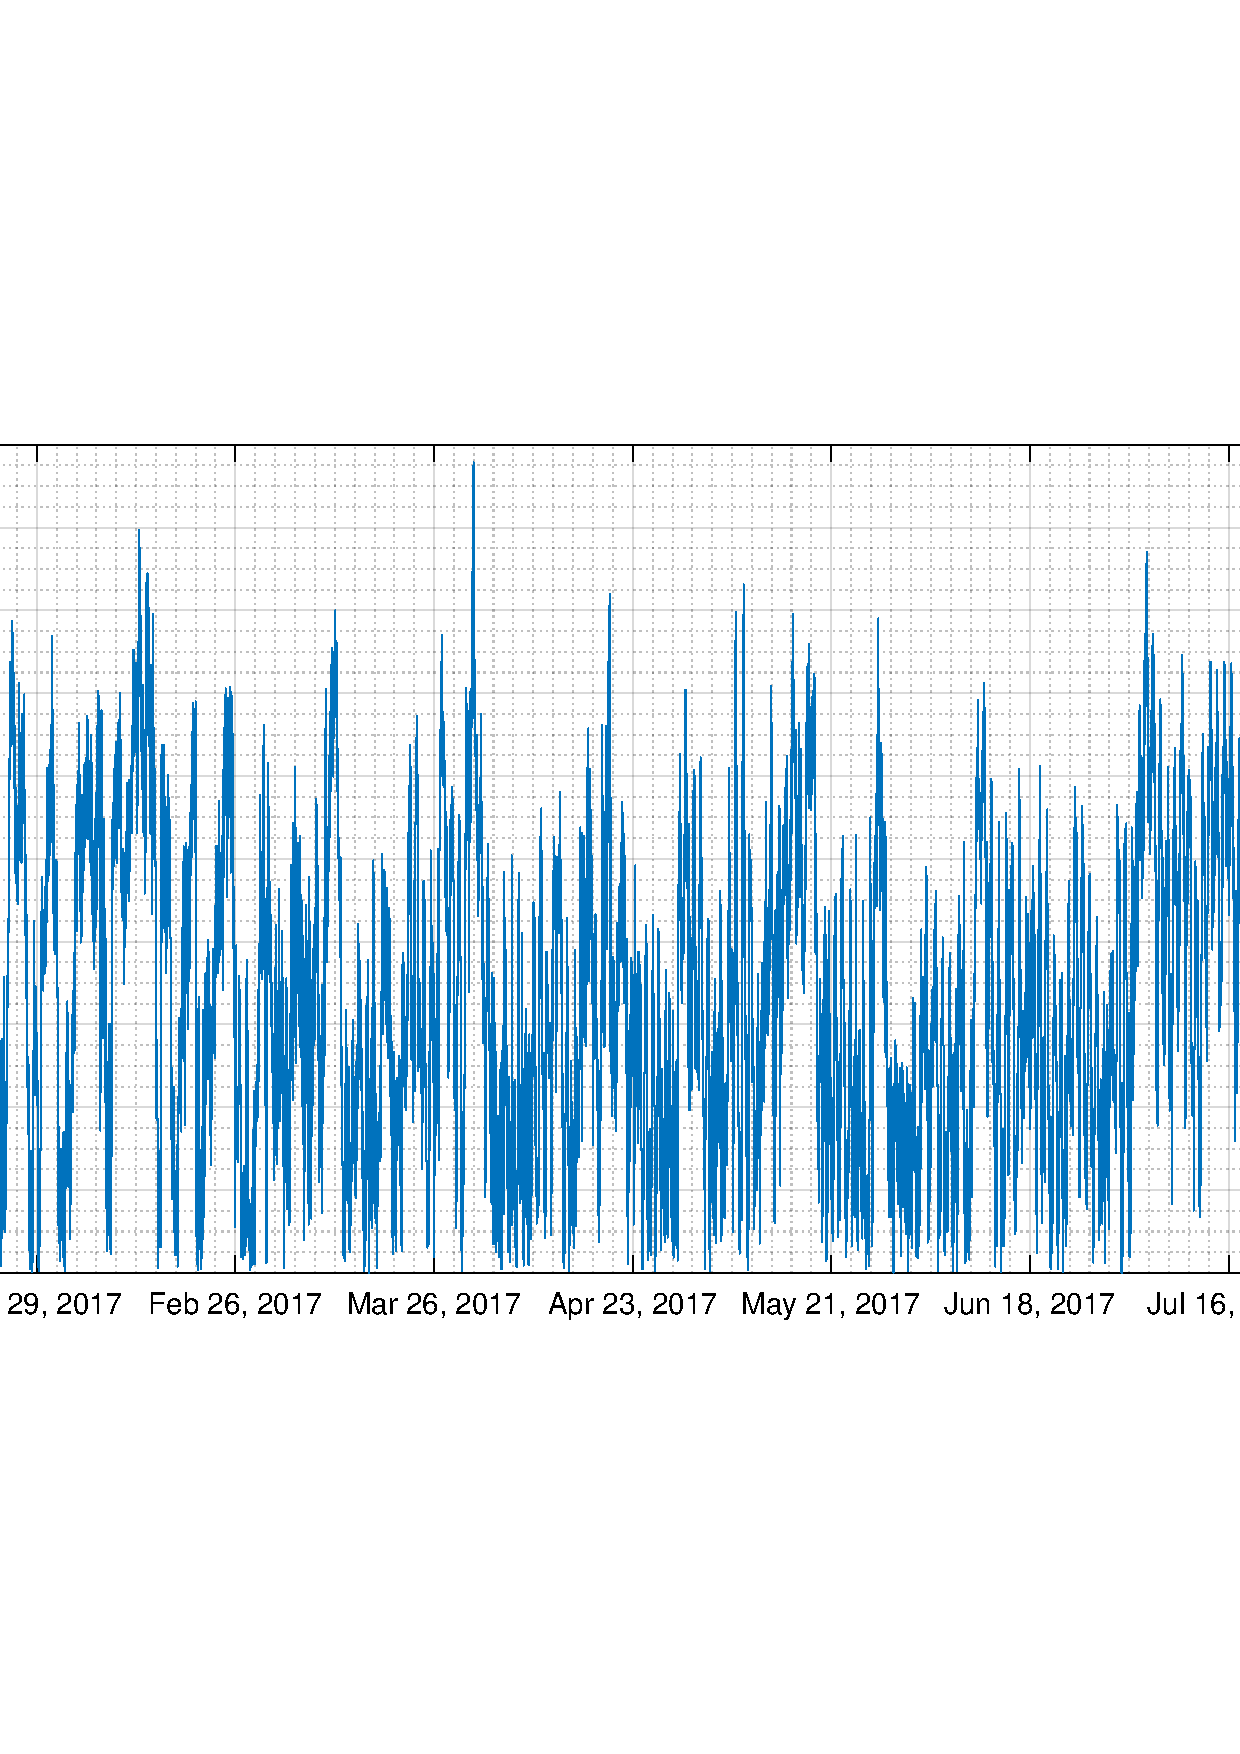
\includegraphics[width=1.\linewidth]{windspeeds.png}
	\caption{Variation of the Wind Speed in the Site}
	\label{windvariation}
\end{figure}
Probability density function (PDF) of the measurements is given in Fig. \ref{windpdf}. The wind speed measurements have a mean of 7.13 with a standard deviation of 3.85.\par
\begin{figure}[h!]
	\centering
	\includegraphics[width=.8\linewidth]{pdf_wind.pdf}
	\caption{Probability Density Function of Measured Wind Speeds}
	\label{windpdf}
\end{figure}
For a defined wind speed, the active power increase can be calculated by considering the Section \ref{sec:klimit}. However, likelihood of such an increase can be calculated by integrating PDF over desired the wind speed range. This can also be calculated from the cumulative distribution function (CDF) of the measurements. In this case, CDFs of the wind speed range limits will be used. Wind Speed CDF is given in Fig. \ref{windcdf}. \par
\begin{figure}[h!]
	\centering
	\includegraphics[width=.8\linewidth]{cdf_wind.pdf}
	\caption{Cumulative Distribution Function of Measured Wind Speeds}
	\label{windcdf}
\end{figure}
By utilizing the wind speed measurements and the possible increase in the active output power, it is possible to define availability of the wind turbine for a possible inertial support. In other words, the increase in the active power can be united with the probability of the corresponding speed. In this way, the contribution from different wind speeds is obtained. The net power contribution for varying wind speed is given in the Fig. \ref{net_contribution}.\par
\begin{figure}[h!]
	\centering
	\includegraphics[width=1\linewidth]{netcontribution.pdf}
	\caption{Distribution of Fast Inertial Support}
	\label{net_contribution}
\end{figure}
First of all, the net contribution when the wind speed is below 3m/s is zero since the turbine is in the cut-off. The probability of the cut-off according to wind speed measurements is found out as 14.16 from the pdf or cdf of the measurements. The main contribution concentrates inside the wind speed range between 3 and 10. Due to the fact that this wind speed range has both higher probability and higher increase capability, the main contribution is provided inside this range. Meanwhile, the higher speed range has relatively lower contribution due to its lower probability and lower capability. \par
Another important criteria is the net contribution from all wind speeds. Since Fig. \ref{net_contribution} is basically product of the pdf given in Fig. \ref{windpdf} and the increase in the active power given in Fig. \ref{increase_active_power}, the area under the graph gives the net contribution from a wind turbine by considering the probability of the each wind speed measurement. Therefore, it can be concluded that the wind turbine studied in this thesis subject is able to provide 0.3pu active power.
\section{Fast Inertial Support Under Different Wind Speeds}
Active power of the wind turbines is determined by parameters such as wind speed, pitch angle and turbine speed. Therefore, combination of these parameters have importance for a possible fast inertial support. In other words, wind turbine under high wind scenario has different potential than that under low wind scenario. Likewise, the resultant states of wind turbines for inertial support would be much different. In this section, the effect of wind speeds will be investigated for fast inertial support. Active power of wind turbines will be increased by different percentages in the fastest way independent of the grid frequency. Turbine internal parameters such as the change in generator speed, turbine and generator torques, DC-link voltage and pitch angle, if any, will be observed. 
\subsection{Low Wind Scenario}
\label{sec:lowwind}
The minimum speed of the wind turbine generator in this scenario is 550 rpm (4.7 rpm in the rotor). Wind speed that will capture the maximum power from wind in this generator speed is found out to be 3.12m/s. In this scenario, the kinetic energy stored in the turbine inertia is minimum and calculated in Eq. (\ref{kineticenergymin}). This scenario investigates the case where the least amount of kinetic energy exists in the turbine equivalent inertia. By the fast inertial support provision, the wind turbine speed decreases below the minimum generator speed. However, the resultant minimum generator speed is dependent on the increase in the active power and also the support interval.
\subsubsection{Fast Inertial Support Limit in Low Wind Scenario}
The electricity grid in the upcoming future might require sudden active power release from wind farms for short time durations to arrest steepest frequency declines. Therefore, it is important to observe the maximum achievable power for inertial support studies. The equation Eq. (\ref{maxxpower}) implies that wind turbine in the low wind speed scenario cannot reach rated active power since the generator speed is much lower than the maximum generator speed. However, the electromagnetic torque in steady state is much lower than the limit torque, $T_{S-lim}$. Therefore, the wind turbine in low speed scenario has the potential for increasing its active power to a significant value. Fig. \ref{low_limit_power} shows the active power, output torque and the speed of the generator. The increase in the active power is obtained by ensuring the limit torque, $T_{S-lim}$. However, since the generator speed is decreasing, the active power is also decreasing due to the fact that further increase in the generator torque is not possible. \par
\begin{figure}[h]
	\centering
	\includegraphics[width=1\linewidth]{low_2000.png}
	\caption{Fast Inertial Support Active Power Limit for Low Wind Scenario}
	\label{low_limit_power}
\end{figure}
Since the turbine is forced to increase its power by high amount compared to pre-disturbance value, the support interval is kept as 1 second. Even in this short duration, the generator speed declines significantly. Variation of the turbine power, $P_{tur}$ and generator power, $P_{gen}$ as well as the generator speed, $\omega_{m}$ is shown in Fig. \ref{low_limit_power}. It is to note that turbine might stall if the support duration is extended. \par
\subsubsection{Moderate Fast Inertial Support for in Low Wind Scenario}
Wind turbines are able to increase its power to significant values even in the low wind speed scenario. However, the time interval is kept as short as possible in order to avoid excessive energy extraction from renewable sources. Nonetheless, the longer support periods can be achievable if the increase in the active power is decreased. Therefore, in this part, the active power of the wind turbine is increased 10\% for three different time intervals as 5, 10 and 20 seconds. The active power output of the wind turbine is given in Fig. \ref{lowactivepowers}. It is observed that turbine power decreases below the nominal value after the support period in order to recover the generator speed. Another observation is the fact that higher support time creates higher dip in the active power in the speed recovery period.\par
\begin{figure}[h]
	\centering
	\includegraphics[width=.9\linewidth]{lowwindpowers.png}
	\caption{Active Power Output of the Wind Turbine for Low Wind Scenario}
	\label{lowactivepowers}
\end{figure}
\begin{figure}[h]
	\centering
	\includegraphics[width=1.0\linewidth]{lowspeeds.png}
	\caption{Generator Speeds of the Wind Turbine for Low Wind Scenario}
	\label{low_speeds}
\end{figure}
Generator speed decreases continuously until the support is ended. The generator speeds are shown in Fig. \ref{low_speeds} for three support times. The decrease in the generator speed is obtained with an increase in the generator torque. The turbine torque, generator torque and generator speed for 5 seconds support is given in Fig. \ref{low_torques}. The generator torque is increased at t=10s for a time duration of 5 seconds. Turbine torque increases slightly with decreasing speed. However, the increase in the turbine torque is negligible when it is compared to the increase in generator torque as shown in zoomed graph. Therefore, the turbine torque can be considered to be constant for the support period meanwhile the generator torque is increased. Turbine and generator torque for 20 second case is also shown in Fig. \ref{low_torques3}.\par
\begin{figure}[h!]
	\centering
	\includegraphics[width=1.0\linewidth]{low_s5_zoomed.png}
	\caption{Turbine Torque, Generator Speed and Torque for 5 Seconds Support under Low Wind Speed}
	\label{low_torques}
\end{figure}
\begin{figure}[h!]
	\centering
	\includegraphics[width=1.0\linewidth]{low_s20.png}
	\caption{Turbine Torque, Generator Speed and Torque for 20 Seconds Support under Low Wind Speed}
	\label{low_torques3}
\end{figure}
When the active power is increased, increased amount of active power is transferred from MSC to GSC. Increased active power should be injected to grid without causing excessive voltage rise on the DC-bus. It is to note that the voltage rise in the very first seconds in inertial support activation is same for all three support cases. However, the voltage drop will be highest in the 20 seconds case. DC-link voltage for 20 seconds support case is given in Fig. \ref{low_vdc_s20}. The rise on DC-bus voltage can be considered as negligible for three support cases.
\begin{figure}[h!]
	\centering
	\includegraphics[width=1.0\linewidth]{low_vdc_20.png}
	\caption{DC-Link Voltage for 20 Seconds Support in Low Wind Speed}
	\label{low_vdc_s20}
\end{figure}
\subsection{Medium Wind Scenario}
In the medium wind scenario, wind turbine operated in the middle of the generator speed range. The medium wind speeds have the huge potential for fast inertial support as stated in the Section \ref{sec:klimit}. Besides, the wind turbine has more kinetic energy than that of low wind scenario and it can reach higher active power values due to its higher MPPT speed. The wind speed is selected as 6m/s in this scenario. 
\subsubsection{Fast Inertial Support Limit in Medium Wind Scenario}
It is already mentioned that wind turbines in the medium wind speed scenario can increase its power more than that of low wind speed scenario. The reason is the dependency of the active power on the generator speed. The active power limit in the medium wind speed scenario is given in Fig. \ref{medium_limit_power}. The wind turbine active power is increased more than 0.4pu as expected in the Fig. \ref{increase_active_power}.\par
\begin{figure}[h]
	\centering
	\includegraphics[width=.95\linewidth]{power_torque_medium_limit.png}
	\caption{Fast Inertial Support Active Power Limit for Medium Wind Scenario}
	\label{medium_limit_power}
\end{figure}
\begin{figure}[h!]
	\centering
	\includegraphics[width=.95\linewidth]{speed_medium_limit.png}
	\caption{Generator and Turbine Power and Generator Speed for Medium Wind Speed Limit Case}
	\label{medium_limit_speed}
\end{figure}
The generator and turbine powers as well as generator speed are depicted in Fig. \ref{medium_limit_speed}. Generator speed decreases due to increased generator power while the turbine power is almost constant. Since the turbine leaves the MPP point, the turbine power declines. However, the change in the turbine power is small. Therefore, the turbine power is said to be constant for this interval. The variation of the DC-bus voltage is shown in Fig. \ref{medium_limit_dc-bus}. The rise in the DC-link voltage is up to 1.04pu and it is regulated in 200ms. 
\begin{figure}[h]
	\centering
	\includegraphics[width=.95\linewidth]{dclinkvoltage_medium_limit.png}
	\caption{Variation of DC-bus Voltage for Medium Wind Speed Limit Case}
	\label{medium_limit_dc-bus}
\end{figure}
\subsubsection{Moderate Fast Inertial Support for in Medium Wind Scenario}
Fast inertial support with a duration of 1 second can be evolved to moderate inertial support with longer duration of support and small incrase in active power. Therefore, the active power of the wind turbine is increased by 10\% and it is shown in Fig. \ref{midpowers} for three different time intervals. The recovery period of shortest support case is much more smoother than the longer ones. When the support time is increased, active power of the wind turbine is almost halved that might cause also problems in frequency stability of the power systems. \par
\begin{figure}[h!]
	\centering
	\includegraphics[width=1.0\linewidth]{medium_powers.png}
	\caption{Active Power Output of the Wind Turbine for Medium Wind Scenario}
	\label{midpowers}
\end{figure}
In medium wind scenario, higher support time causes decreased active power after the support. The reason is the lower speed value obtained with higher support time. Generator torque is decreased much higher for this case in order to recover the speed. \par
The generator speed, turbine and generator torques are shown in Fig. \ref{mid_torques3}. After the support, MPPT algoritm takes action and regulates the speed correspondingly. Therefore, the generator torque jumped down to lower value to restore the MPPT speed. The negative jump in generator torque crates a negative jump in the active power of the wind turbine since the transferred power is the multiplication of generator torque and generator speed.\par
\begin{figure}[h!]
	\centering
	\includegraphics[width=1.0\linewidth]{medium_s20.png}
	\caption{Generator Speed, Generator and Turbine Torques for Medium Wind Scenario for 20 Seconds Support}
	\label{mid_torques3}
\end{figure}
The fast inertial support is activated in time 10 seconds. The rise on the DC-bus voltage is negligible as in the case of low wind scenario. However, the voltage drop at the end of support is much more significant than that of low wind scenario. The variation of DC-bus voltage with inertial support is shown in Fig. \ref{med_vdc_s20} for the 20 seconds support case.
\begin{figure}[h!]
	\centering
	\includegraphics[width=1.0\linewidth]{medium_s20_vdc.png}
	\caption{DC-Link Voltage for 20 Seconds Support in Medium Wind Speed}
	\label{med_vdc_s20}
\end{figure}
\subsection{High Wind Scenario}
In this section, wind turbine operation with high wind speed is investigated. The high wind scenario is much different than the low and medium wind speed scenarios. Firstly, the wind turbine injects its maximum power to grid. Secondly, the generator reference speed is the maximum allowable speed, $\omega_{max}$ which implies that wind turbine operation is away from MPPT operation. In order to keep the generator in the maximum available speed, the pitch angle is used in order to curtail wind power. The reason for using pitch angle is that the generator torque is limited by $T_{P-lim}$. Therefore, the wind turbine decreases turbine power and torque by increasing pitch angle. The wind speed in this scenario is selected as 11.4m/s.\par
\subsubsection{Fast Inertial Support Limit in High Wind Scenario}
Wind turbines are able to provide inertial support in high wind speed as long as converter power rating is higher than the wind turbine generator power rating. The wind turbine investigated throughout the study has a converter rating of 3.04MVA meanwhile turbine power rating of 2.75MW. Therefore, active power output can be increased up to 3.04MW during support interval as long as the converter and generator handle excess losses due to overloading. Otherwise, wind turbine cannot provide inertial support for high wind speeds. In the low and medium wind scenarios, the active power can be increased much higher than 10\% in the limit case. However, the limit and moderate fast inertial support cases are the same for high wind speed scenario and limited by 10\%. The active power is increased to its limit for 1 second duration as shown in Fig. \ref{high_powers}. The generator torque is increased from 1pu to 1.1pu. The increase in the torque rises the power to the maximum allowed power rating. However, the increase in the currents causes excess heat and mechanical stress on the wind turbine generator, gearbox and the power converters. Therefore, the support period should be limited as well as the next possible support should be delayed. \par
\begin{figure}[h]
	\centering
	\includegraphics[width=1\linewidth]{highwindpowers.png}
	\caption{Fast Inertial Support Active Power Limit for High Wind Scenario}
	\label{high_powers}
\end{figure}
Turbine and generator powers, generator speed and pitch angle is shown in Fig. \ref{high_limit_speed}. The turbine power in this case rises with the inertial support that is different than low and medium wind scenarios. Moreover, the speed starts decreasing with the support. However, as the generator speed declines below the maximum generator speed, pitch angle of the turbine blades decreases. Therefore, the fast inertial support does not require speed recovery since the speed is recovered as soon as the power goes back to pre-disturbance value. \par
\begin{figure}[h]
	\centering
	\includegraphics[width=1 \linewidth]{speed_high_limit.png}
	\caption{Turbine and Generator Powers, Generator Speed and Pitch Angle for High Wind Limit Scenario}
	\label{high_limit_speed}
\end{figure}
\begin{figure}[h!]
	\centering
	\includegraphics[width=1 \linewidth]{dclinkvoltage_high_limit.png}
	\caption{Variation of the DC-bus Voltage for High Wind Limit Scenario}
	\label{high_limit_dcbus}
\end{figure}
Finally, the DC-bus voltage is shown in the Fig. \ref{high_limit_dcbus}. The reason of the rise on DC-bus is the unbalance between generator power and power injected to grid. In other words, rise on the DC-bus voltage is directly linked to the additional power. The quicker the grid power is increased, the lower DC-bus voltage rise is obtained. Since the increase in the active power to the limit is lowest in the high wind scenario, DC-bus voltage rise is lower than that of the low and medium wind scenarios. \par
\subsubsection{Moderate Inertial Support Limit in High Wind Scenario}
In this part, the active power of the wind turbine is increased again by 10\% with three different time intervals. The active powers are shown in Fig. \ref{high_powerss}.\par
\begin{figure}[h!]
	\centering
	\includegraphics[width=1.0\linewidth]{high_s5_10_20_power.png}
	\caption{Active Power Output of the Wind Turbine for High Wind Scenario}
	\label{high_powerss}
\end{figure}
An interesting observation in high wind scenario is that there is no speed recovery process. As soon as the speed is decreased, the pitch controller decreases the blade angle which causes an increase in turbine torque. Therefore, in this case, turbine power decreases back to normal rather than a lower power value as in the other scenarios. In the high wind scenario, the generator torque hits the limit defined for normal operating conditions. This is why generator speed is regulated with the help of blade angle. Therefore, pitch angle is also important in this section. \par
Generator speed, turbine and generator torques as well as pitch angle for 20 seconds support case is shown in Fig. \ref{high_s20}. Generator speed starts decreasing when the generator torque is increased. However, the pitch controller decreases the blade angle since the generator speed is below the maximum speed. Therefore, the generator speed rises when the pitch angle is decreased. Note that pitch servo acts slower than the generator torque increase time. This is why the generator speed decreases until the pitch angle is decreased. Generator speed might not be disturbed if the pitch controller is able act fast enough.\par
After the generator speed is arrested by the pitch angle decrease, generator speed rises towards the maximum generator speed. If the support time is increased, the generator speed will reach the maximum speed, and will stay constant with a new pitch angle. This means that the turbine is able to provide the support forever. However, the full capacity of the converter cannot be used permanently since it causes  overloading of the converters in the wind turbine and excess heat losses. Therefore, maintaining permanent support would be dangerous. Finally, the rise on the DC-bus voltage is the same with the high speed limit case meanwhile the voltage drop at the end of the support period might increase with the duration. Nonetheless, the detailed modelling of the DC-bus voltage with the actual converter parameters would give the most realistic results for this study.
\begin{figure}[h!]
	\centering
	\includegraphics[width=1\linewidth]{torques_speed_pitch_20s.png}
	\caption{Pitch Angle, Generator Speed, Generator and Turbine Torques for High Wind Scenario for 20 Seconds Support}
	\label{high_s20}
\end{figure}
